\documentclass{article}


\usepackage{amsmath} % math stuff
\usepackage{amssymb} % math stuff
\usepackage{array} % equations and stuff
\usepackage{bm} % bold math
%\usepackage{caption} % suppressed table numbering; incompatible with revtex, and longtable, I think
\usepackage{comment} % comment environment
%\usepackage{enumitem} % customization of enumeration, itemize, and description
\usepackage[T1]{fontenc} % font encoding for special characters, must also use scalable font package
\usepackage[margin=0.8in]{geometry} % paper sizes and margins (but be careful not to mess up pre-defined pages)
\usepackage{graphicx} % for graphics
%\usepackage{helvet} % default font is the helvetica postscript font
\usepackage{lipsum} % lorem ipsum filler text
\usepackage{lmodern} % scalable font?
\usepackage{longtable} % multi-page tables
\usepackage{mathrsfs} % math script font
\usepackage{mhchem} % easier chemical formula
\usepackage{microtype} % allows disabling of ligatures
%\usepackage{newcent} % new century schoolbook font
\usepackage{nicefrac}
\usepackage{parskip} % removes paragraph indentation, and adjusts paragraph skip, as well as list items
%\usepackage{setspace} % adjust text spacing and indents
\usepackage{siunitx} % decimal alignment
\usepackage{subfigure} % divided figures
%\usepackage{tabu} % extra table options
\usepackage{textcomp} % symbols
\usepackage{threeparttablex} % better footnotes with longtable
\usepackage{titling} % title placement
\usepackage{ulem} % strikethrough text
%\usepackage{url} % superceded by hyperref
\usepackage{verbatim} % verbatim environment
\usepackage{xcolor} % colors and color boxes
\usepackage{xspace} % commands that don't eat up white space
\usepackage{hyperref} % links and page setup; should always come last

\hypersetup{
	bookmarks=true,
	colorlinks=true,
	citecolor=blue,
	linkcolor=blue,
	urlcolor=blue,
	pdfstartview={XYZ null null 1.0} % default open view is 100%
}

\DisableLigatures[f]{encoding = *, family = * } % disable ff, fi, fl ligatures, without f option, it also disables -- = endash
\renewcommand{\arraystretch}{1} % extra vertical space in tables

\begin{document}

\pagestyle{empty} % don't number pages

% custom title
\begin{center}
{\LARGE Express Riddler}

\vspace{0.15in}

{\Large 22 May 2020}
\end{center}


\section*{Riddle:}

To share a cylindrical muffin equally with his two toddlers, Robert makes three vertical cuts in a ``Y'' pattern, producing three equal pieces.

The next morning, his wife wants in on the fun. But before he can cut the muffin into quarters with an ``X'' pattern, one of his children suggests using an ``A'' pattern.
If Robert were to produce equal fourths in this manner, what would be the ratio of length of the A's middle bar to the radius of the muffin?

\section*{Solution:}

This is a pretty straightforward geometry problem.
The cuts basically look like this (not to scale):

\vspace{0.1in}
\begin{center}
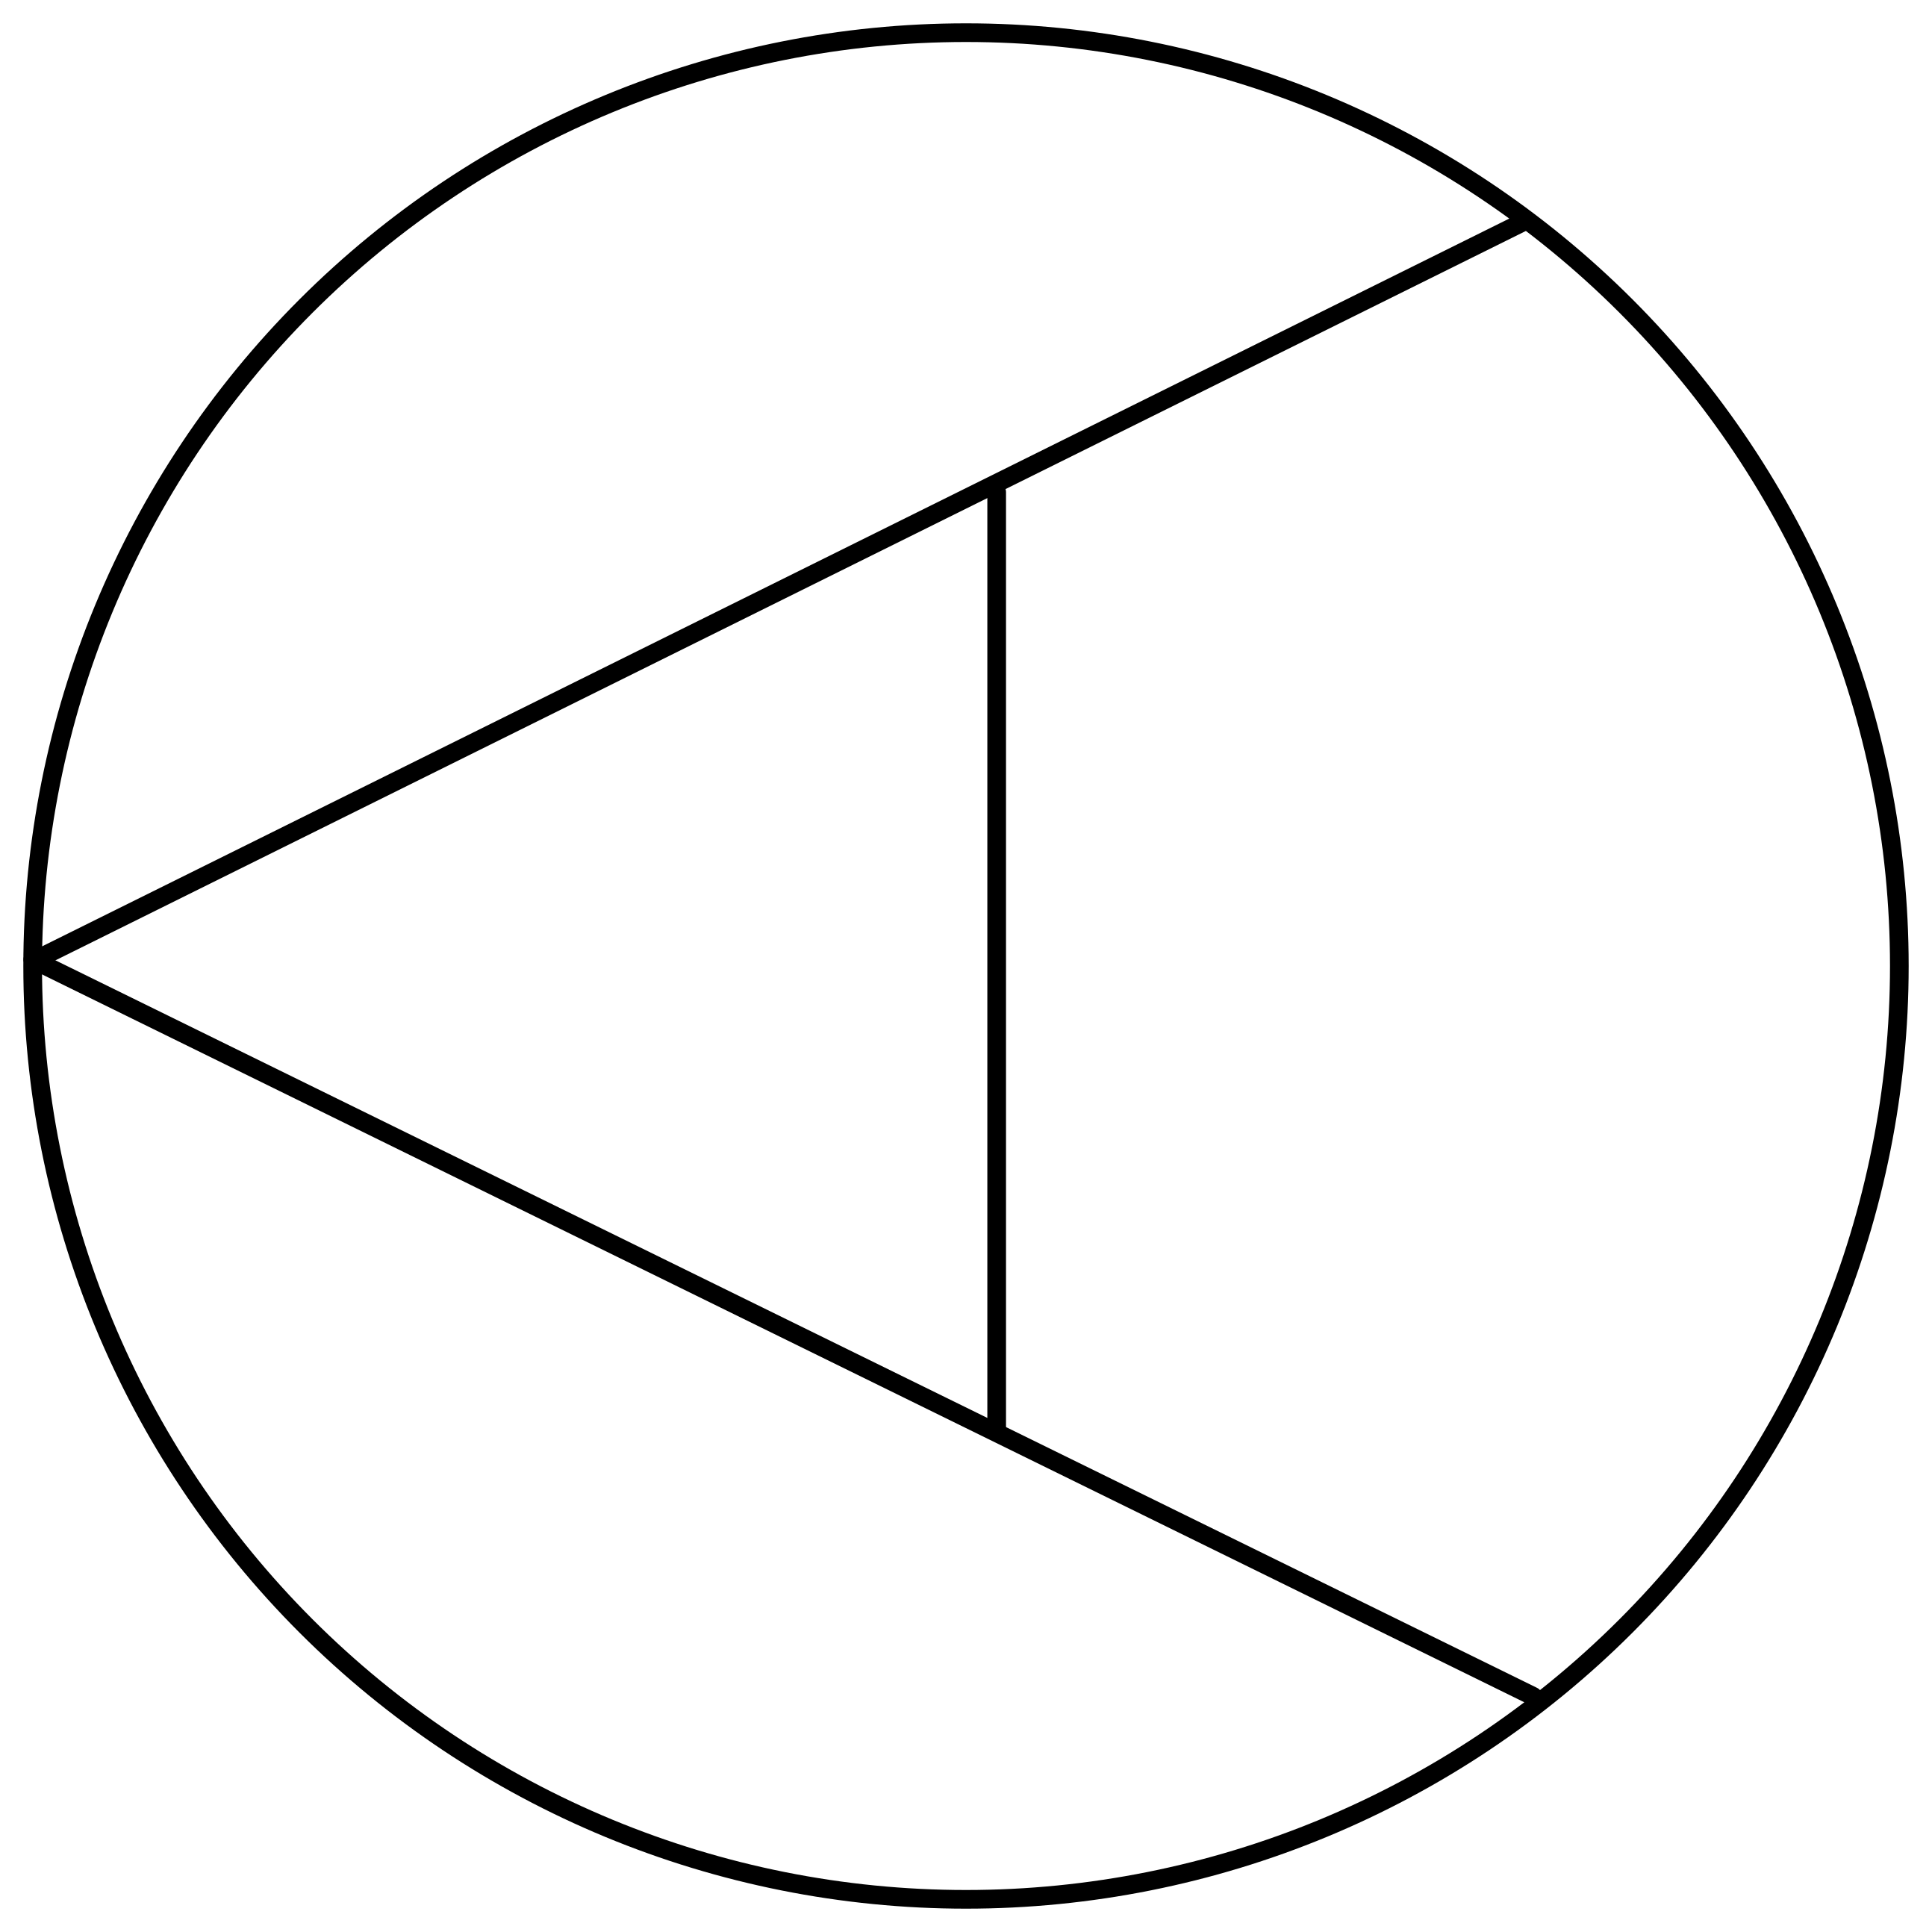
\includegraphics[width=2.5in]{A_cut.png}
\end{center}
\vspace{0.1in}

The first thing to calculate is the angle of the two secant cuts, which create two rounded cuts, each with area $\nicefrac{\pi}{4}$.
Although the area of these two regions is not immediately clear, it is simply the difference of two more easy-to-calculate areas.
For this calculation I used the following scheme:

\vspace{0.1in}
\begin{center}
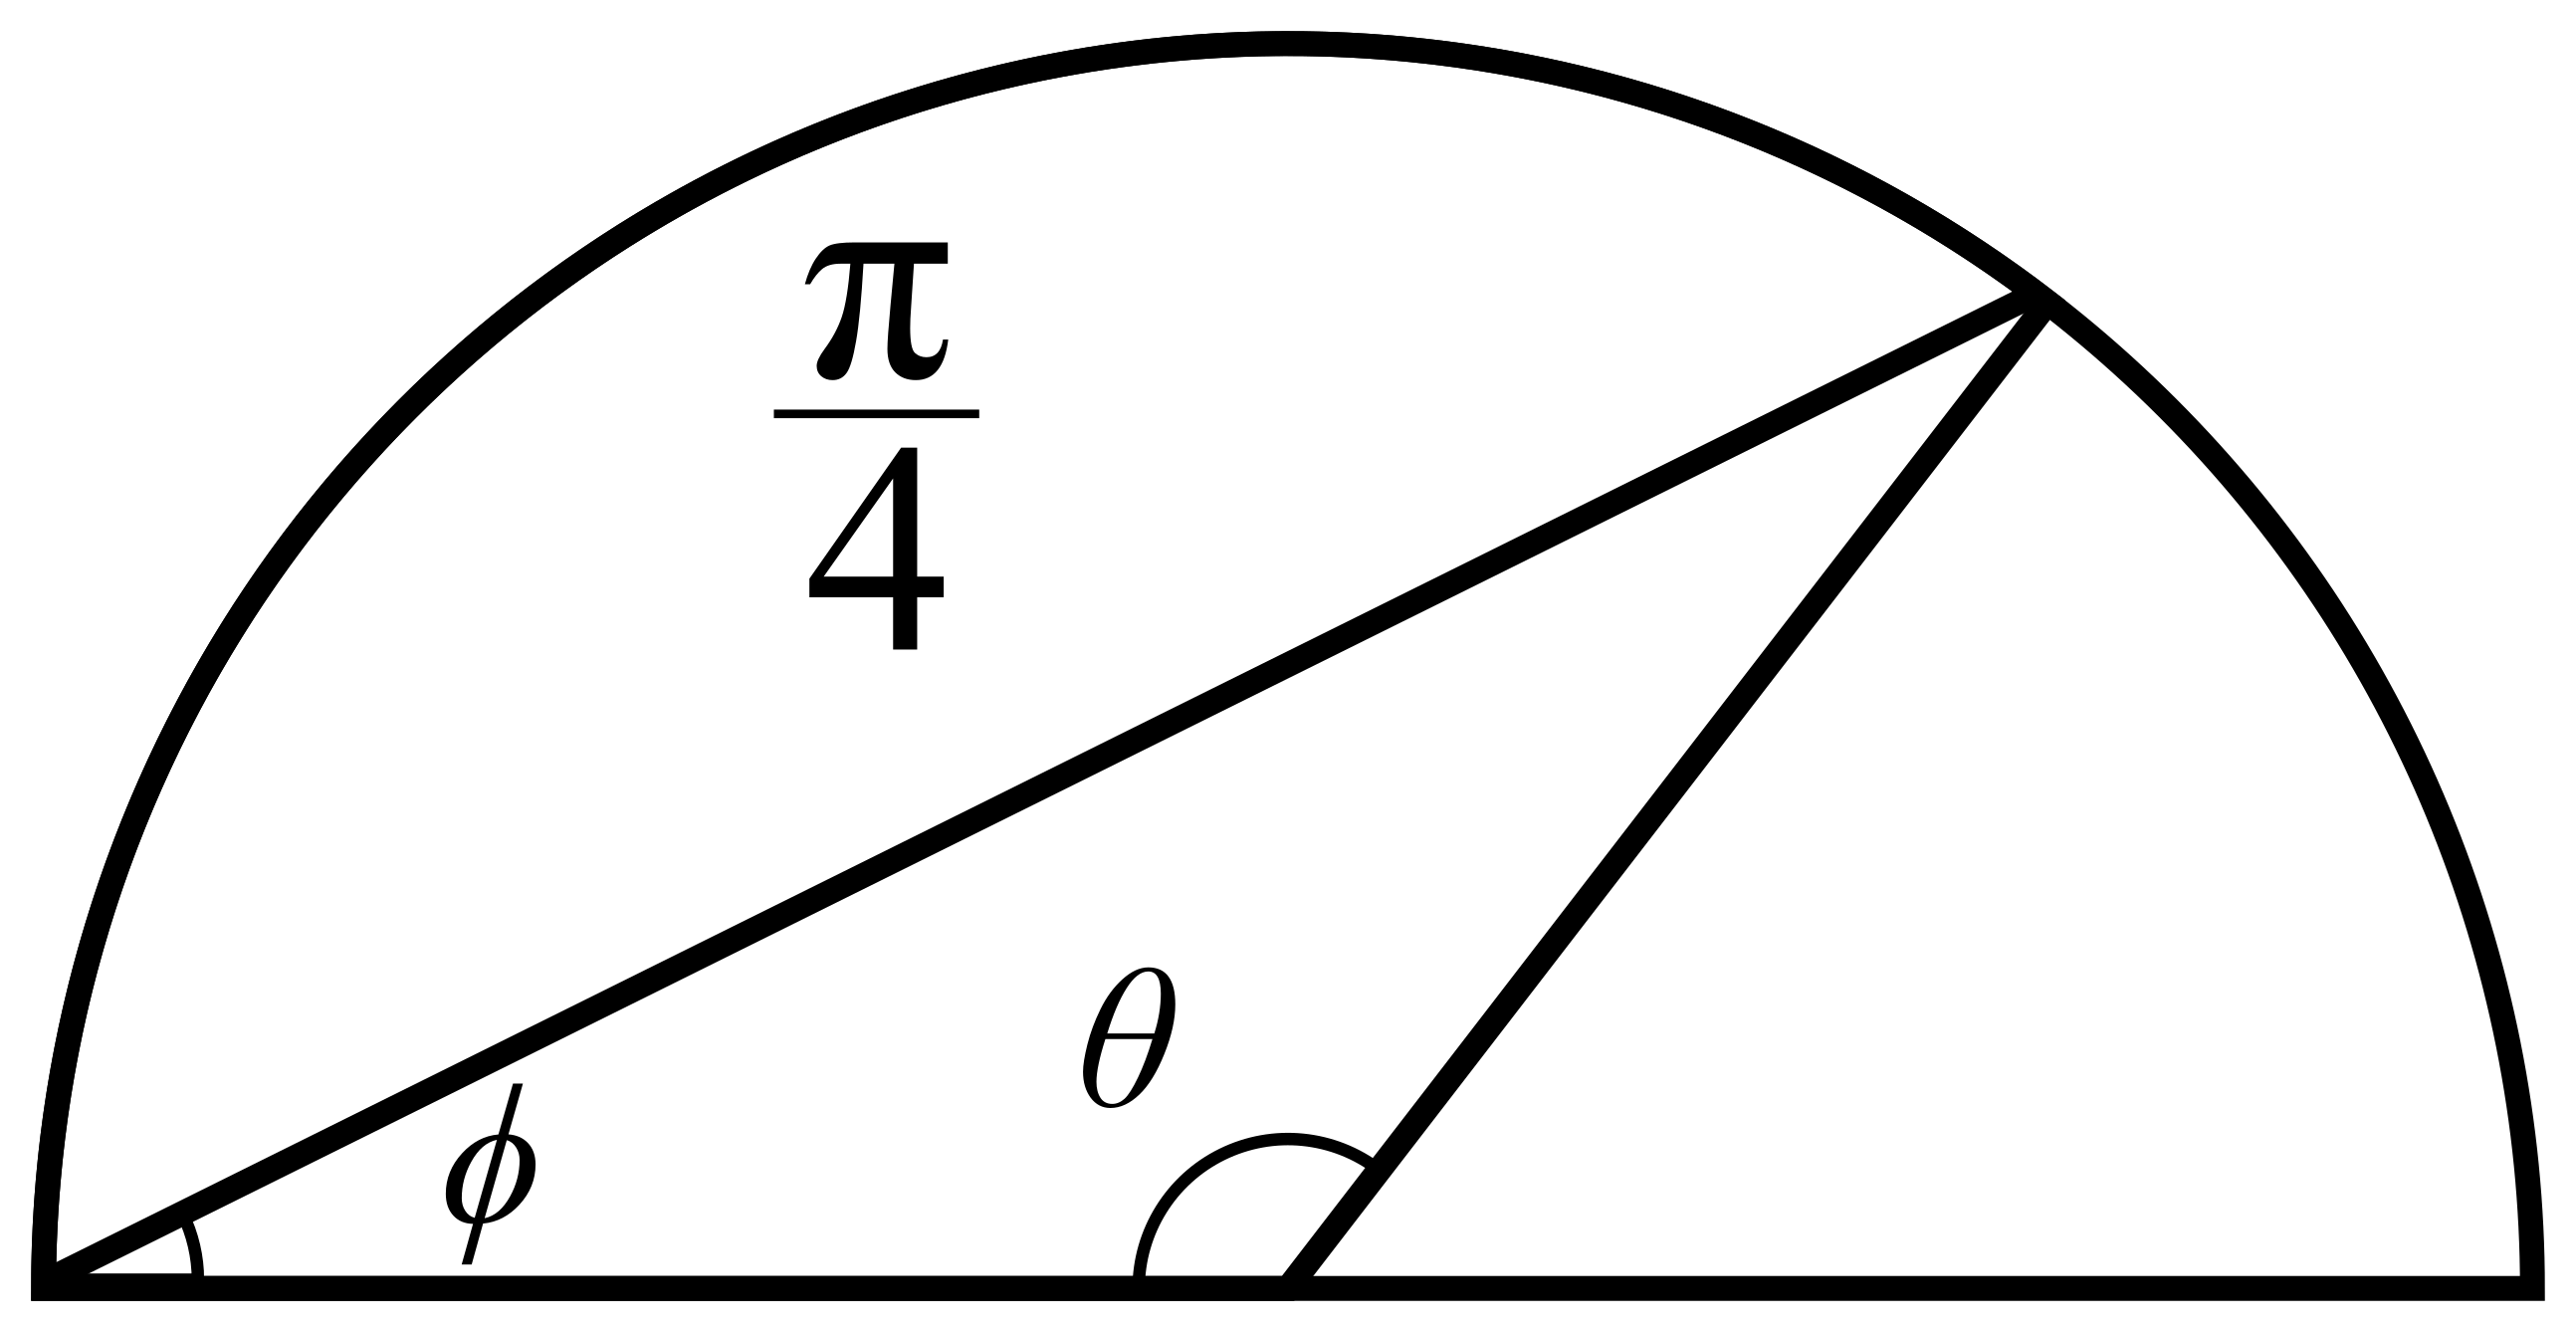
\includegraphics[width=2.5in]{first_cut.png}
\end{center}
\vspace{0.1in}

For an obtuse triangle sitting along the radius of a unit circle, its base is simply 1, and the height is just $\sin\theta$.
Thus the area of the triangle is $(\nicefrac{1}{2})\sin\theta$.
The area of the whole arc including the triangle is $(\nicefrac{\theta}{2\pi})\pi=\nicefrac{\theta}{2}$.
Then the difference of the two areas, which is what we need, is $\nicefrac{\theta}{2}-(\nicefrac{1}{2})\sin\theta=\nicefrac{\pi}{4}$, which gives $\theta\approx\ang{132.5}$.

Now it is important to note that because the triangle is isosceles, the angle $\phi$ can be calculated as $\theta+2\phi=\ang{180}$, which gives $\phi\approx\ang{23.83}$.
From here, the third can be calculated, which divides the remaining center piece in half.
I have used these dimensions to calculate the size of this cut:

\vspace{0.1in}
\begin{center}
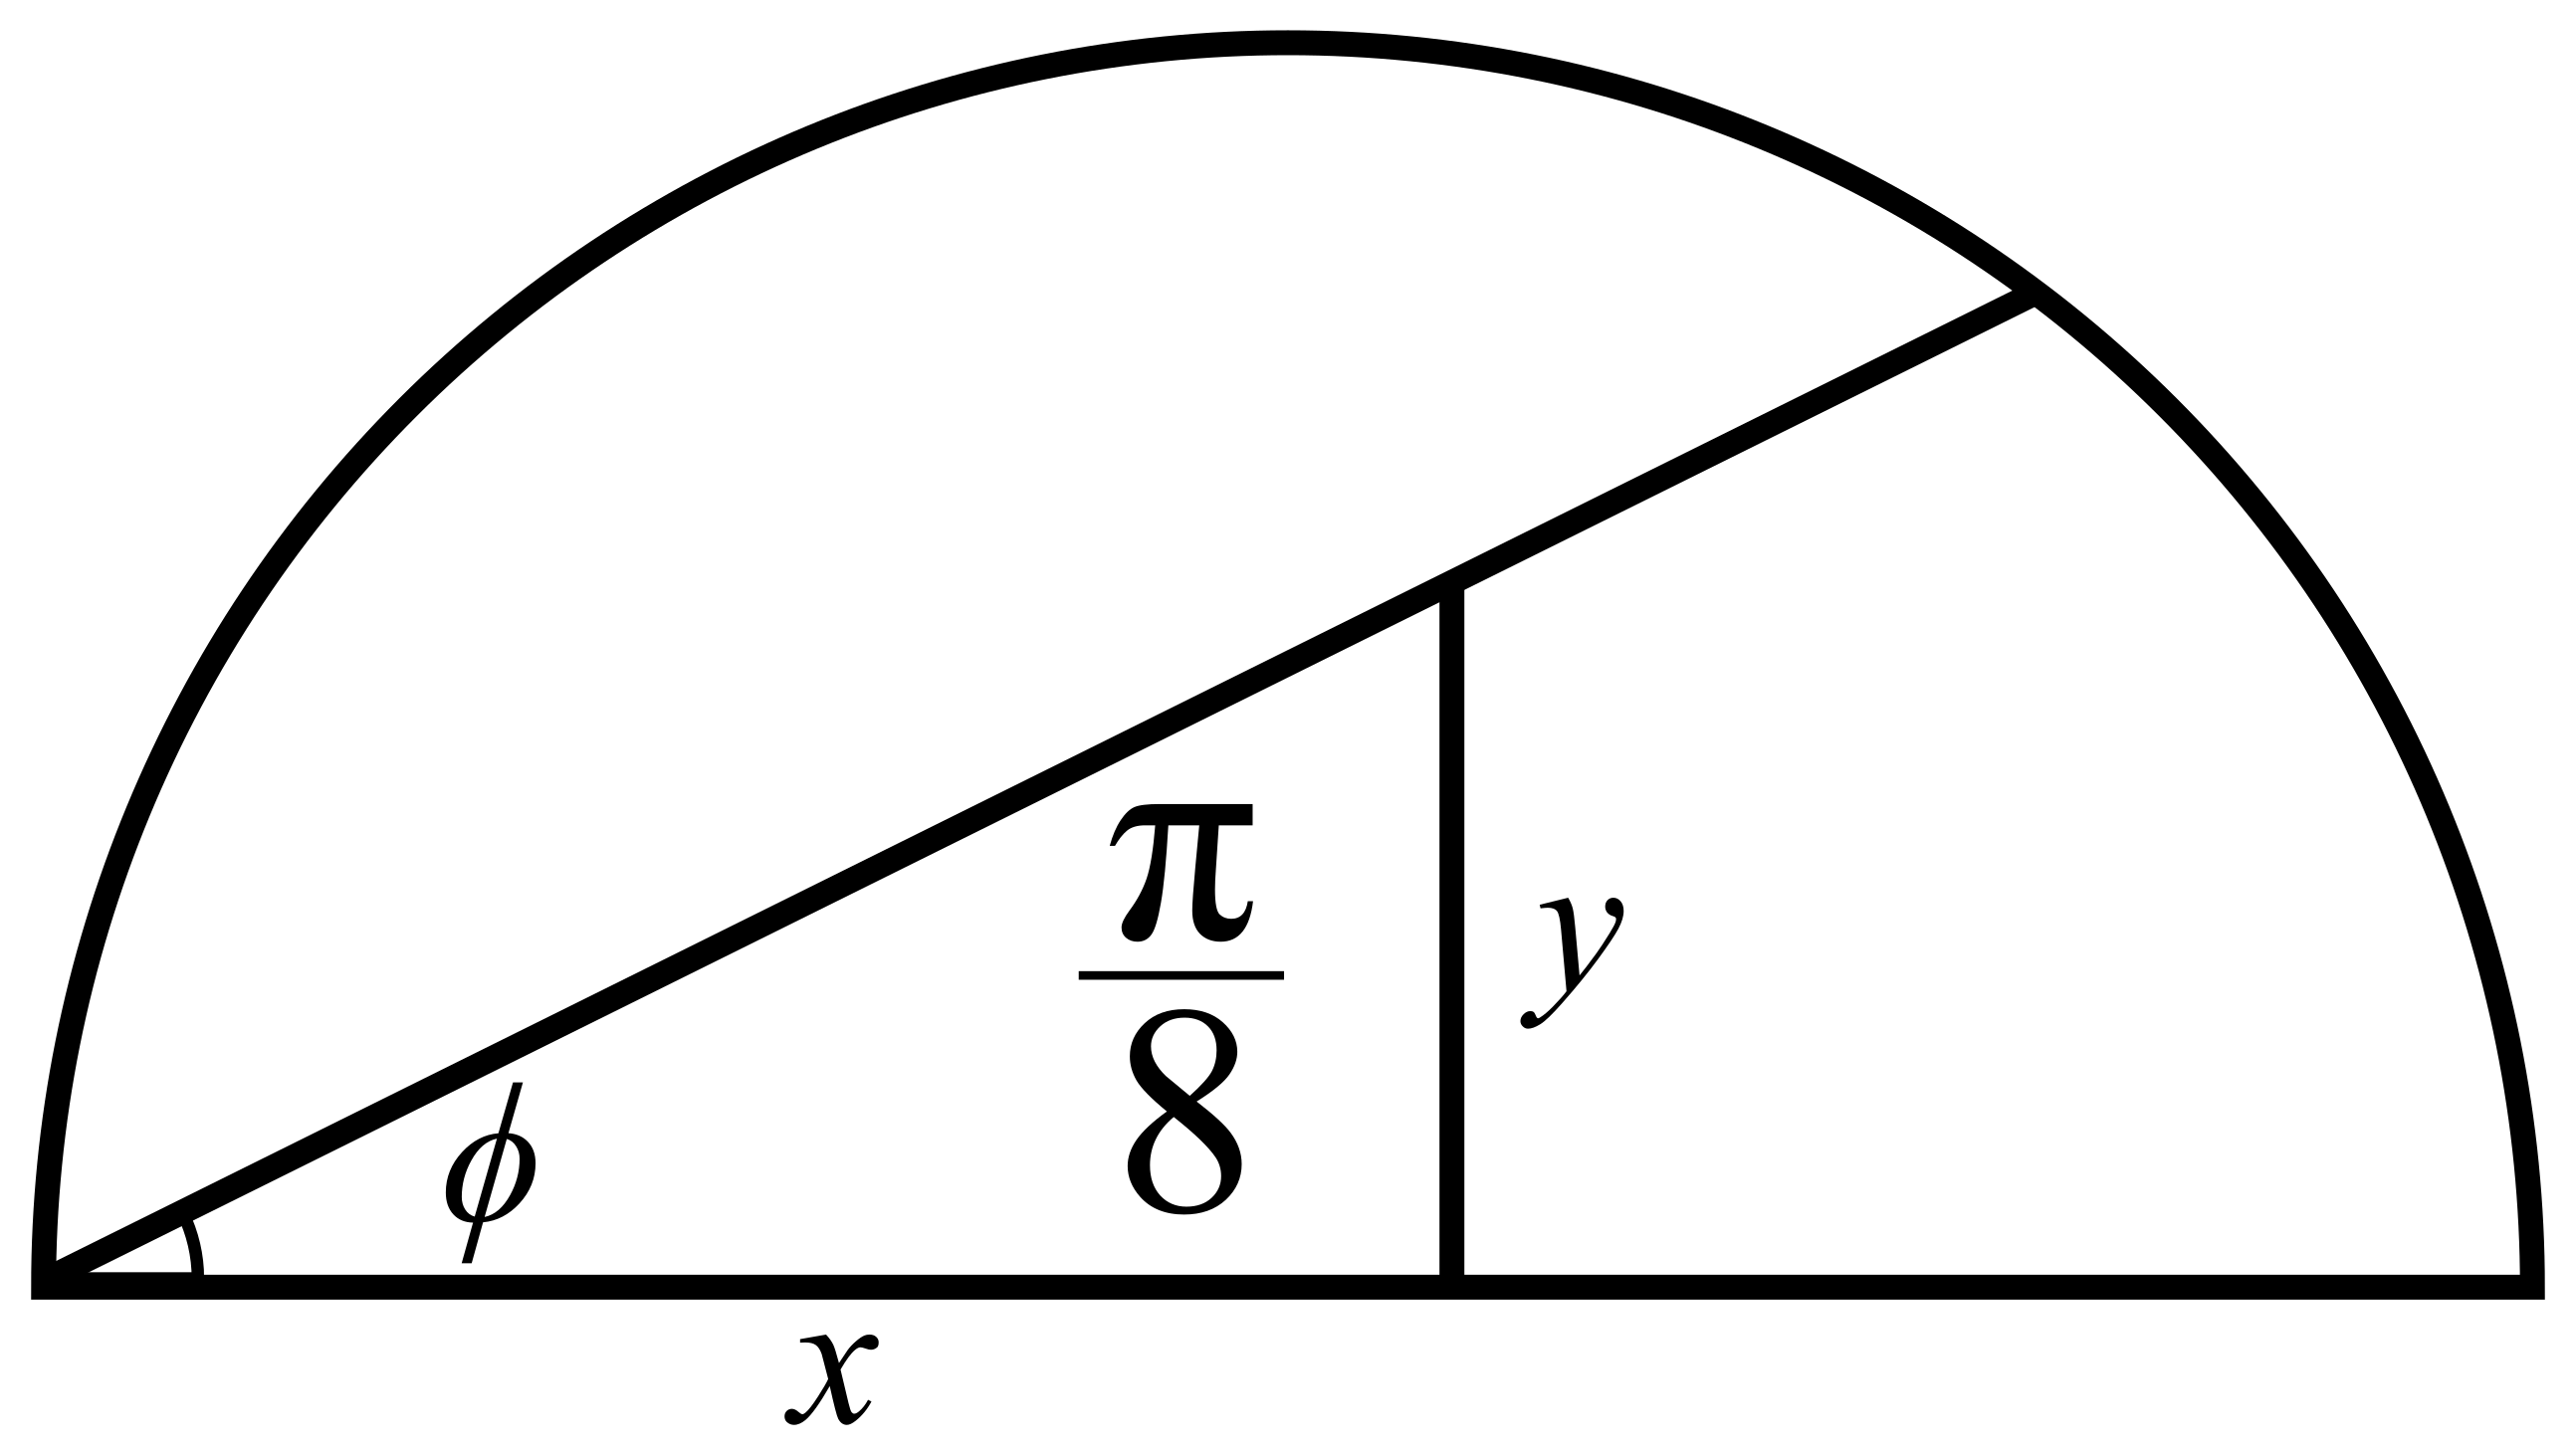
\includegraphics[width=2.5in]{second_cut.png}
\end{center}
\vspace{0.1in}

We need to solve for $y$ because that is the length about which the riddle is asking.
It is easy to see that $x=y\cot\phi$.
Then the area of the triangle is $(\nicefrac{1}{2})y^{2}\cot\phi=\nicefrac{\pi}/8$, which gives $y\approx0.5890$.
The full length of the cut is twice this value, so the solution is (approximately)
\fcolorbox{red}{white}{\bf 1.178}\,.



\end{document}